\documentclass[a4wide]{article}
\usepackage{a4wide}
\usepackage{appendix}
\newcommand{\comment}[1]{{\tt #1}}
\usepackage{graphicx}
\usepackage{listings}
\usepackage[section]{placeins}
\title{RocketMouse:\\ OO Software System Design}

\author{Hesham H. Salman \and Jonathon Kissinger \and Sean Mead \and Troy Johnson}

\begin{document}
\maketitle


\section{External Design Specifications}
The design for layout for the user game will be relatively simple. When the user launches the game, if they have already filled out the initial survey, they will be presented with the menu in figure ~\ref{fig:intro_image} in the appendices. If the user hasn't filled out the initial survey, they are presented with a survey they must fill out before navigating to the menu in figure ~\ref{fig:intro_image}. This menu will give the user several options. The user will have the option play the game, view details about the creators of the game, and check the results of their data that was most recently sent in for processing. If the user selects to play the game, they will be presented with a layout similar to that of figure ~\ref{fig:screen_layout} in the appendices. This is the game layout the user will be presented with when they select the button to start actually playing the game.



Figure ~\ref{fig:screen_layout} in the appendices is the basic game layout. However, more details may be added later if time permits. The design will be a two-dimensional side scroller game in which the user is represented by a character of some sort (a stick figure in our case in figure ~\ref{fig:screen_layout}) in the appendices. The user will then have to jump over some type of object that pops up as the user moves along from left to right across the screen. A figure of the user jumping can be seen in figure ~\ref{fig:user_jumping} in the appendices.



 The time it takes from when a block first appears, to the time it takes the user to tap the screen to make their character jump over the block is what we will use as the  measure for reaction time for the user. Once the user has finished playing, their reaction times are uploaded to the server for further processing. Once their results have been processed and analyzed and the results are received on the user's mobile device, the user will see a screen similar to that of figure ~\ref{fig:diagnosis_screen} in the appendices, where they are notified about their results.

The results of our data mining of their response time data may become more detailed later on depending upon how accurate we can get with our prediction models. For now, we will just have them a low,medium, or high recommendation for getting checking out by a doctor for the possibility of a ADHD diagnosis.

\section{Architectural Design Specifications}

\subsection{Functional Model}
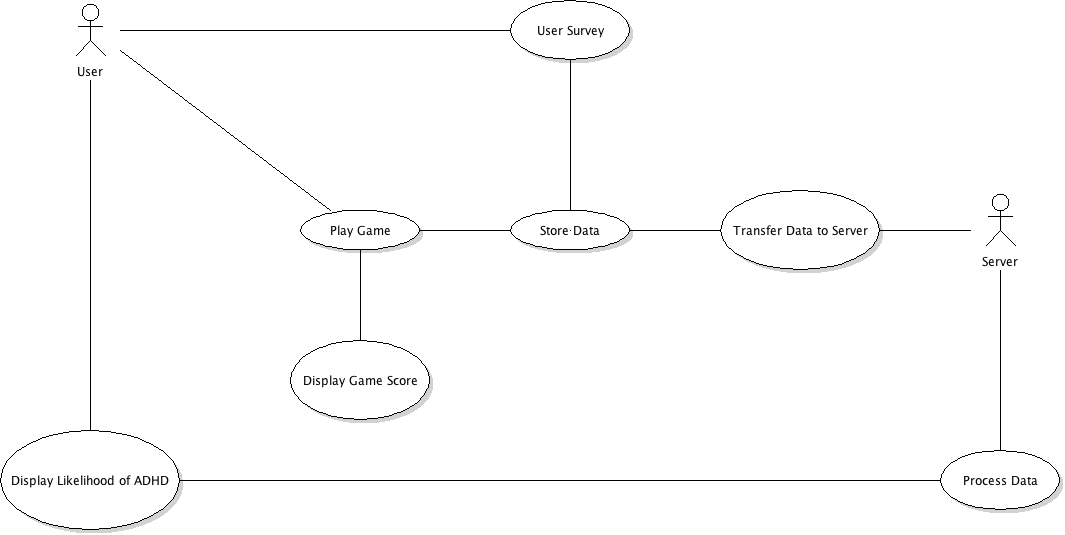
\includegraphics[width=\textwidth]{images/UseCaseDiagram.png}
\small Fig. 1: Use Case Diagram involving user and server actions
\subsection{State Diagram}
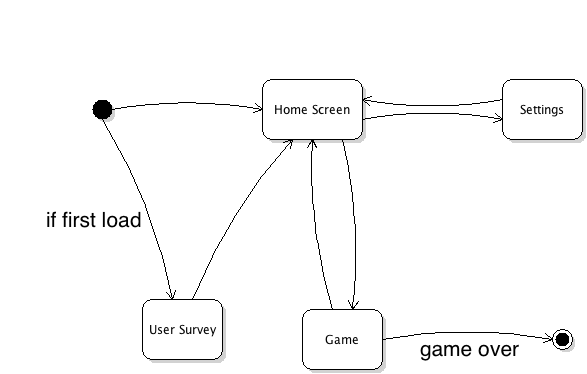
\includegraphics[width=\textwidth]{images/StateDiagram.png}
Fig. 2: State Diagram for RocketMouse
\subsection{Dynamic Model}
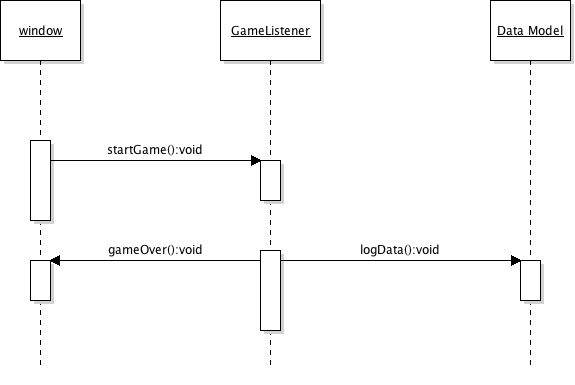
\includegraphics[width=\textwidth]{images/dynamicModel.png}
Fig. 3: Dynamic Model for RocketMouse
%%%%%%%%%%%%%%%%%%%%%%%%%%%%%%%%%%%%%%%%%%%%%%%%%%%%%%%%%%%%%%%%
\section{Detailed Design Specifications}

\subsection{Interface Specifications}
\begin{itemize}
\item public interface SyncInterface\newline
- Relays the results of the sync to the calling thread.
\end{itemize}

\subsection{Class Definitions}
\begin{itemize}
\item class AddAppsTask extends AsyncTask\newline
- Adds applications to the main sqlite database.
\item class AddResultTask extends AsyncTask\newline
- Adds results from gameplay to the main sqlite database.
\item class SyncTask extends AsyncTask\newline
- Syncs the list of applications and gameplay results with the server.
\item public class SyncService extends Service\newline
- Controls timed executions of the SyncTask.
\item public class MainDatabase extends SQLiteOpenHelper\newline
- Controls thread-safe access to the database.
\item Request Library\newline
- The Request Library consists of numerous abstractions for thread creation, tcp communication and object transmission.
\begin{itemize}
\item public class Client extends DefaultHttpClient\newline
- Registers custom ssl connections.
\item public class ClientManager implements ClientStatusController\newline
- Abstracts the thread-safe creation of ThreadedClient
\item public class NameValueBuilder\newline
- Used to abstract form creation for POST requests.
\item public class Request\newline
- Abstracts the creation and execution of threaded network tasks.
\end{itemize}
\end{itemize}


\subsection{Algorithms}
Gathering Applications and adding them to the database.
\begin{lstlisting}
List<ApplicationInfo> appInfoList = pm.getInstalledApplications(PackageManager.GET_ACTIVITIES);
List<Application> appList = new ArrayList<Application>();
for(Application app: appList){
	mdb.addApp(app);
}
\end{lstlisting}

\begin{lstlisting}
long start = MainDatabase.getHelper(context).getMinimumDate();
long stop = System.currentTimeMillis();
		
boolean didCache = false;	//whether the cache/caches have uploaded properly
boolean didSync = false;	//whether the current master db/dbs have uploaded properly
		
String srcPath = MainDatabase.getHelper(context).getPath();		//file path of the master database
		
long startSync = Epoch.getDayEpoch(start);		//floor the requested range to the start of the day
long stopSync = Epoch.getDayEpoch(stop);
		
if(stopSync>System.currentTimeMillis()){		//hopefully not an issue... will check and deny going back to the future.
	Log.d("CACHE",String.valueOf(didCache));
	Log.d("SYNC",String.valueOf(didSync));
	return false;
}
if(startSync==stopSync){						//check to see if the upload will be pointless
	return false;
}

long cacheStart = startSync;		//make a copy of the start date because we want to manipulate it
int days = Epoch.getDays(cacheStart,stop,Epoch.MILLIS);		//the total number of days we want to upload

for(int d = 0; d < days; d++){
    FullParser fp = new FullParser();
    String dbPath = fp.build(context, (cacheStart), cacheStart + DAYMS);		//completely parse one full day and return the path
	cacheStart += DAYMS;
	Log.d("CACHE",d+ " PATH: "+dbPath);
			
	//at this point we have a single day cached and ready to upload
	//we will try up to the value of ATTEMPTS times to upload this file
			
	for(int i = 0; i < ATTEMPTS; i++){
		if(ClientManager.connect().status){						//if we have connected to the server
			if(ClientManager.cache(dbPath).status){			//if the server says the cache file is ok
				didCache = true;
				i = ATTEMPTS;
			}
		}
	}
	if(!context.deleteDatabase(dbPath)){
		context.deleteDatabase(dbPath);				//cleanup the file we created
	}
}
		
//at this point all cache creation and uploads are complete

if(!context.deleteDatabase(tdbPath)){
context.deleteDatabase(tdbPath);			//cleanup
}

Log.d("COPY",String.valueOf(didCopy));
Log.d("CACHE",String.valueOf(didCache));
Log.d("SYNC",String.valueOf(didSync));

return didCache&&didSync;
\end{lstlisting}

\subsection{Data file specifications}

Gameplay results and application data will be stored in a sqlite database locally on the mobile device.  That database will sync with our server and will likely be deleted from the device.  One table will be created for the application data and another for the gameplay data.


%%%%%%%%%%%%%%%%%%%%%%%%%%%%%%%%%%%%%%%%%%%%%%%%%%%%%%%%%%%%%%%%
\section{Test Plan}
\begin{enumerate}
\item Performance tests
\begin{enumerate}


\item a.	User interface
\begin{enumerate}
\item	Ease of use - Ask those unfamiliar with the project, and no more than a beginner’s knowledge of the game to attempt to play the game. Ask user on how they think the game could be improved or what may have confused them.
\item	Ease of use on touch device – Make sure icons work fine on touch devices, i.e, make sure that all click-able icons that are used, aren't so small that a user with rather large fingers would have trouble playing the game.
\item	Compatibility with other iOS operating system versions – Mobile game application should be compatible with at least iOS 8.0 or higher. This means that the mobile game will have to be tested on mobile devices with a variety of iOS version above 8.0.
\item 	Other design goals as needed (as more detail is added to the SRS)
\end{enumerate}
\item	Overall system
\begin{enumerate}
\item	 Response time should be quick. No more than 1 second without feedback to the user on their results. Wait times that are required to be longer than that should show a dialog giving an estimated wait time if possible, and a general spinner waiting dialog if not, to show that the app is retrieving or uploading data [1].
\item	Availability – System should always be available other than when maintenance is being performed on the server. Test what happens if the system is shut down while a client is actively playing the game and/or uploading the results of their game. Other than when the server/system is down for maintenance, the system should always be up and running and therefore a user playing the game at any time should be able to upload the data from their game at almost any time.
\item	Security - Normal security measures; to test this we could possibly invite a person with hacking knowledge to attempt to hack the server to obtain personal data. Also, gather advice on the security aspects from security professionals  and ask them what we could do to increase the security of the system.
\item	Recovery - How does the system respond if the client’s connection is lost when uploading the user’s data to the server?
v.	Other design goals as needed (as more detail is added to the SRS)
\end{enumerate}

\item	Stress tests
\begin{enumerate}
\item	Manual - A test where 10 (hopefully more depending on how many testers we can get) logged-in users perform the same functions and see if any wait times or ramp up times occur. This test will help determine how the server reacts to periods of time where many people may be submitting their response time data to the server at the same time for processing.
\item	Automatic - Set up a testing scenario with some open source software testing tool that can simulate as many simultaneous connections as needed (hundreds? thousands?), similar to an integration test. This can method can also be used to determine the maximum number of concurrent users that the server can support under a given configuration.
\item	Automatic - (Similar style as mentioned in b) – Perform a long-running stress test that drives a continuous load on the server for an extended period of time.  (Due to time constraints “long-running” may only consist of a week at most) The main purpose of this type of test would be to ensure the server accepting the data can sustain acceptable levels of performance over an extended period of time without exhibiting any slowdowns.
\item	Use anteater to simulate thousands of pseudo random presses in places on the game screen and see if the application can handle it or to see if it crashes the application.
\end{enumerate}
\end{enumerate}
3.	Functional tests
\begin{enumerate}
\item	Specific test cases:
\begin{enumerate}
\item	User submits response time data with no connection to the server currently available.
\item	User loses connection in the middle of uploading their data to the server.
\item	User uploads their same data to the server multiple times.
\item	User is the first to submit their data to the server (no data to compare against to help determine ADHD diagnosis).
\item	User quits in the middle of the game, make sure data isn’t submitted.
\item	User doesn't give permission to upload their information.

\end{enumerate}
\end{enumerate}
\end{enumerate}

\section{References}
[1]Nielson, Jakob. "Response Times: The 3 Important Limits." Nielsen Norman Group. Nielsen Norman Group, 1 Jan. 1993. Web. 23 Oct. 2014.
\section{Appendices}

\begin{figure}
\centering
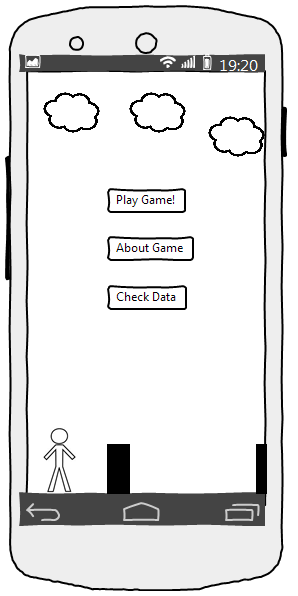
\includegraphics[height=10cm, width = 5cm]{images/intro.png}
\caption{Menu screen user uses to navigate}
\label{fig:intro_image}
\end{figure}


\begin{figure}
\centering
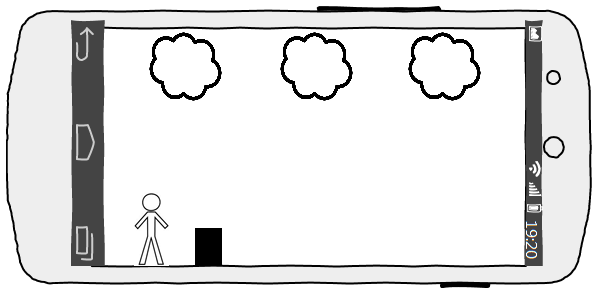
\includegraphics[height=5cm, width = 8cm]{images/screen_layout.png}
\caption{Typical screen layout for user playing game}
\label{fig:screen_layout}
\end{figure}

\begin{figure}
\centering
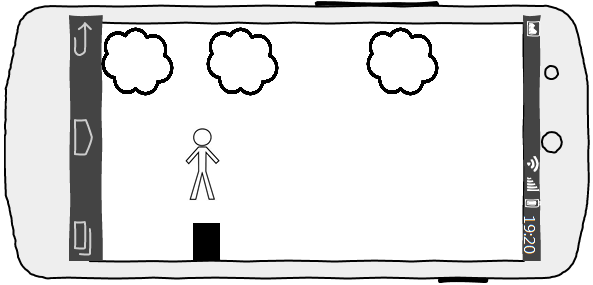
\includegraphics[height=5cm, width = 8cm]{images/user_jumping.png}
\caption{User will have to jump over some type of objects}
\label{fig:user_jumping}
\end{figure}

\begin{figure}
\centering
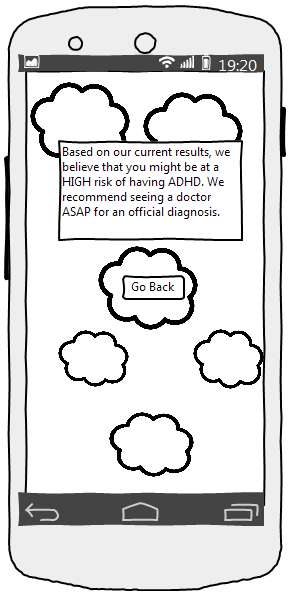
\includegraphics[height=10cm, width = 5cm]{images/diagnosis_screen.png}
\caption{Screen where the user can view their results}
\label{fig:diagnosis_screen}
\end{figure}

\section{Gantt Chart}
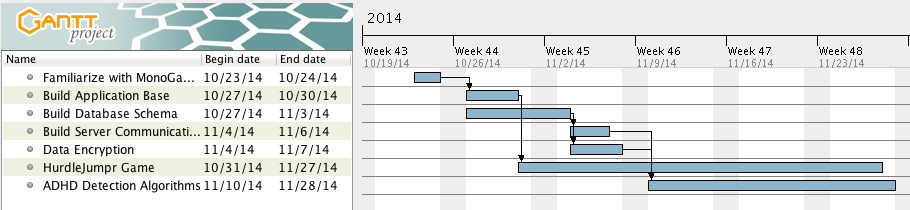
\includegraphics[width=\textwidth]{images/Gantt.png}
\end{document}
